%\subsection{Objectives}
%
%The purpose of the experiment is to show the following points:
%\begin{itemize}
%\item the learning engine produces *accurate* and *concise* descriptions compared to a human
%expert's descriptions but costs just a fraction of the time; 
%\item it handles a variety of data formats; 
%\item the refinement step significantly improves the structure; 
%\item it is able to produce a description that is sufficiently accurate with 
%much smaller training sets (overfitting vs. underfitting); 
%\item demonstrate that there exists a correlation between sample size, execution time and accuracy,
%and the min sample size required to achieve certain accuracy correlates with the 
%data complexity.
%\end{itemize}

We conducted a series of experiments to study the learning algorithm
and measure its performance. In this section, we will show that
\begin{itemize}
\item the learning engine is capable of handing a variety of data formats;
\item while the initial structure discovery generates a reasonably
good candidate, the refinemnt phase siginificantly improves the
quality of the description through rewritings; 
\item the final output of the learning system is highly competitive
when compared with descriptions written by a human expert 
in terms of accuracy and conciseness; 
\item it is possible to learn from a small training set and produce
a relatively accurate description at a fraction of the cost;
\item there exists a positive correlation between the structural complexity
of the data and the minimum training size required to achieve certain
accuracy.
\end{itemize}

\subsection{Preliminaries}
\begin{table*}
\begin{center}
\begin{tabular}{|l|c|c|c|c|c|c|c|l|} \hline
Data source	& Chunks & Bytes	& Mode  &Header	& Array	& Group & Msgs 	& Comments \\ \hline \hline
1967Transactions.short	& 999	& 70929	& line	& no	& no	& no	& no	& transaction records \\ \hline
MER\_T01\_01.cvs	& 491	& 21731 & line  & yes	& no	& yes	& no	& comma-separated records\\ \hline
ai.3000		& 3000		& 293460 & line	& no	& no	& yes	& no	& web log of Amnesty International \\ \hline
asl.log &	1500	& 279600	& line	& no	& no	& yes	& no	& log file of Mac ASL \\ \hline	
boot.log	& 262	& 16241		& line	& no	& no	& no	& yes	& Mac OS boot log \\ \hline
crashreporter.log & 441	& 50152 	& line	& no	& no	& no	& yes	& original crashreporter daemon log \\ \hline
crashreporter.mod & 441	& 49255		& line	& no	& no	& no	& yes	& modified crashreporter daemon log \\ \hline
dibbler.1000	& 999	& 142607 	& line	& yes	& yes	& no	& no	& AT\&T phone provision data \\ \hline
ls-l.txt	& 35	& 1979		& line	& yes	& no	& no	& no	& Stdout from Unix command ls -l \\ \hline
netstat-an	& 202	& 14355		& block	& yes	& no	& no	& no	& output from netstat -an \\ \hline
page\_log	& 354	& 28170		& line	& no	& no	& no	& no	& printer logs \\ \hline
quarterlypersonalincome & 62	& 10177	& line	& yes	& no	& yes	& no	& spread sheet \\ \hline
railroad.txt	& 67	& 6218		& line	& yes	& yes	& yes	& no	& US rail road info \\ \hline
scrollkeeper.log & 671	& 66288		& line	& no	& no	& no	& yes	& log from cataloging system \\ \hline
windowserver\_last.log & 680	& 52394	& line	& no	& no	& no	& yes	& log from LoginWindow server on Mac \\ \hline
yum.txt		& 328	& 18221		& line	& no	& no	& no	& no	& log from package installer Yum \\ \hline
\end{tabular}
\caption{Benchmark profile} \label{tab:benchmarks}
\end{center}
\end{table*}

The original data sources we used in the experiments are listed in Table \ref{tab:benchmarks}.
These range from personal spread sheet, to government records to system logs, and 
represent vastly different formats. Some benchmarks are large with a few thousand
chunks or records, while others are small with just a few dozen lines. As we will see later
that the size of the data source has some implications in the training performance.
Most of the data files are line based, which means a line represent a data record, with
the exception of netstat-an in which data come in blocks or multiple lines.
Many of the formats include headers or footers which may complicate the descriptions.
From a human point of view, dibbler.1000 and railroad.txt consist of some special
character separated arrays. The ``Group'' column in the table shows if a data source
contain groupings delimited by special characters such as [, ], or quotations.
The ``Msgs'' column indicates whether the data source contains complex English text.
We include two versions of crashreporter.log: an original file ``crashreporter.log''
and ``crashreporter.log.mod'' with some of the date information replaced by ``-''. 
The latter has been used as an example in Section \ref{sec:review}. 

The system that executed the experiments is an 
Apple PowerBook G4 with a 1.67 GHz Processor and 512 MB DDR RAM 
running on Mac OS X 10.4 Tiger. 

\begin{table}
\begin{center}
\begin{tabular}{|l|c|c|c|} \hline
		&  Time to prod.	& MDL score 	& Parsing accuracy 	\\ \hline
HW IR	& -			& X		& -			\\ \hline	
HW PADS	& X			& -		& X			\\ \hline	
INF IR 	& -			& X		& -			\\ \hline
INF PADS & X			& -		& X			\\ \hline 
\end{tabular}
\caption{Measurement for the representations} \label{tab:metrics}
\end{center}
\end{table}

For any of the given data sources, there exists four different representations in 
our experiments: hand-rewritten PADS by human expert (HW PADS), hand-rewritten IR directly
translated from the HW PADS (HW IR), inferred IR from the learning engine (INF IR), and
inferred PADS description which is automatically translated from the INF IR (INF PADS). 
Note that as IR has a simplified language and is not as powerful as the full-fledged
PADS, the HW PADS does not use those features not available in IR and hence it is
not fully optimized. 
Nonetheless, the HW PADS and HW IR are thought to be ``pretty good'' descriptions of
the data and are used as control in the comparisons below. 
In general, we measure the time to produce the descriptions, the MDL scores of
and the parsing accuracy of the descriptions. 
Table \ref{tab:metrics} shows what we measure for each of the four representations.

\subsection{Experiments}
\begin{table*}
\begin{center}
\begin{tabular}{|l||r|r|r|r||r|r|c|} \hline
Formats 	 & Inf time (s) 	& Ref time (s) 	& Total time (s) & HW time (h) & Inf score 	&Ref score	& HW score \\ \hline \hline
1967Transactions.short & 0.20&      2.32&      2.56 	& 4.0 & 0.295 	&0.218 		&0.268		 \\ \hline
MER\_T01\_01.csv & 0.11&      2.80&      2.92 	& 0.5 & 0.648 	&0.112		&0.138		 \\ \hline
ai.3000          & 1.97&      26.35&     28.64	& 1.0 & 0.503	&0.332		&0.338		 \\ \hline
asl.log          & 2.90&      52.07&     55.26	& 1.0 & 0.630	&0.267		&0.361		 \\ \hline
boot.log         & 0.11&      2.40&      2.53 	& 1.0 & 0.620	&0.481		&0.703		 \\ \hline
crashreport.log   & 0.12&      3.58&      3.73 	& 2.0 & 0.607	&0.328		&0.348		 \\ \hline
crashreport.log.mod & 0.15&      3.83&      4.00 	& 2.0 & 0.612	&0.329		&0.347		 \\ \hline
dibbler.1000     & 2.24&      5.69&      8.00 	& 1.5 & 0.602	&0.470		&0.438		 \\ \hline
ls-l.txt         & 0.01&      0.10&      0.11 	& 1.0 & 0.559	&0.333		&0.401		 \\ \hline
netstat-an       & 0.07&      0.74&      0.82 	& 1.0 & 0.413	&0.394		&0.319		 \\ \hline
page\_log        & 0.08&      0.55&      0.65 	& 0.5 & 0.540	&0.107		&0.353		  \\ \hline
quarterlypersonalincome & 0.07&      5.11&      5.18 	& 48  & 0.544	&0.367		&0.354		\\ \hline
railroad.txt     & 0.06&      2.69&      2.76 	& 2.0 & 0.715	&0.506		&0.522		 \\ \hline
scrollkeeper.log & 0.13&      3.24&      3.40 	& 1.0 & 0.625	&0.354		&0.352		 \\ \hline
windowserver\_last.log  & 0.37&      9.65&      10.07	& 1.5 &0.618		&0.241		&0.267		 \\ \hline
yum.txt          & 0.11&      1.91&      2.03 	& 5.0 &0.827		&0.305		&0.474		 \\ \hline
\end{tabular}
\caption{Main results (Inf: structure inference, Ref: Refinement, HW: Hand-written)}
\label{tab:results}
\end{center}
\end{table*}

We first hand-coded all 16 formats in PADS and IR and measure timings and the scores 
of supposedly good descriptions (see HW time column in Table \ref{tab:results}). 
Several formats takes a few hours and up to 2 days(!) to complete because these were the very first 
PADS descriptions ever written by this person. It is obvious that coding description
in PADS is a daunting task for a novice despite that he is a computer science PhD!
To score a given HW IR, we wrote a simple recursive-descent parser with backtracking
for our IR so that the original data can be populated into the IR structure for
correct scoring of the data complexity which is the second component of the MDL score.
After a few attempts and modifications, the HW PADS descritions parses all 
the original data files with 100\% accuracy.

Next we ran the learning system on all 16 data files in their entirety, 
measured timings for structure inference, refinement and the total time which includes
printing out the PADS descriptions and other overhead. 
For accurate timing measurements, run each data format 10 times, and take the average 
after removing the best and the worst times.
We also recorded the scores of both the initial structure and the final structure after refinement.
All these measurements are included in Table \ref{tab:results} as well.
The generated PADS descriptions parses all original data files with 100\% accuracy,
therefore the correctness of the learned formats is guaranteed.

We can see from Table \ref{tab:results} that the learning system
generates correct descriptions of any given data in matters of seconds as opposed to
the hours and days taken by human beings. The execution time is roughly proportional
to the size of input data. For example, the largest data sources, ai.3000 and asl.log,
take also the longest time. Refinement typically takes more time than initial
structure discovery, as the functional dependency analysis in this phase is a quadratic
in the number of nodes in the IR and is the bottleneck of the algorithm. 
Note that all these timings are achieved with a completely unoptimized prototype system
with lots of overhead in book-keeping and I/Os.

%Compare these with the golden numbers from (1) in a big table. Show that the difference in scores
%can be siginificant in some cases hence room for improvement (may go into the discussion section)
%but timing advantage is huge and refinment improves initial struct a lot. Maybe also compare a case or
%two where the score from silver is comparable to golden and the actually description produced is also
%close to golden (to demo that our scoring makes some sense).
%Have a discussion here about while the learning tool may produce a longer description than human does,
%it parses all data correctly so the user is getting all these for free which is a tremendous benefit.
%Discuss 1967 where the inference does better than human.

Select random training sets of 5\%, 10\%, 15\%, ..., 80\% of 
the original data (3 sets for each size) and run learning tool end to end on 
them and take the average of 3 sets. 
Set threshhold levels of 90\% and 95\% accuracies and record how much training data (in percentage and
absolute terms) is needed for each golden format to achieve these accurary levels. Then relate this
to the normalized type complexty of the inferred IR of the entire data sets.
Plot graph of (timing, accuracy) vs. training size 
for a few examples, and show that we are doing a good job with reasonable sample size. The diagram should
show increasing accuracy and execution time as sample size goes up. Point out anomaly
where the abolute training size is too small (e.g. for ls-l.txt which only has 35 lines) which results
in overfitting. ls-l.txt is also problematic as it has a header in the first line and if that is not included
in the training set, the data will not parse.

\begin{figure}
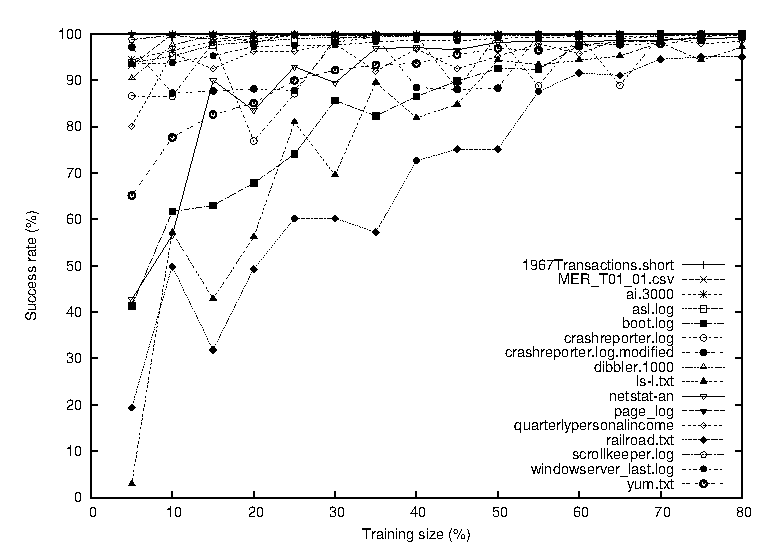
\epsfig{file=successrate.eps, width=\columnwidth}
\caption{Success rates of training sets}
\end{figure}

\begin{figure}
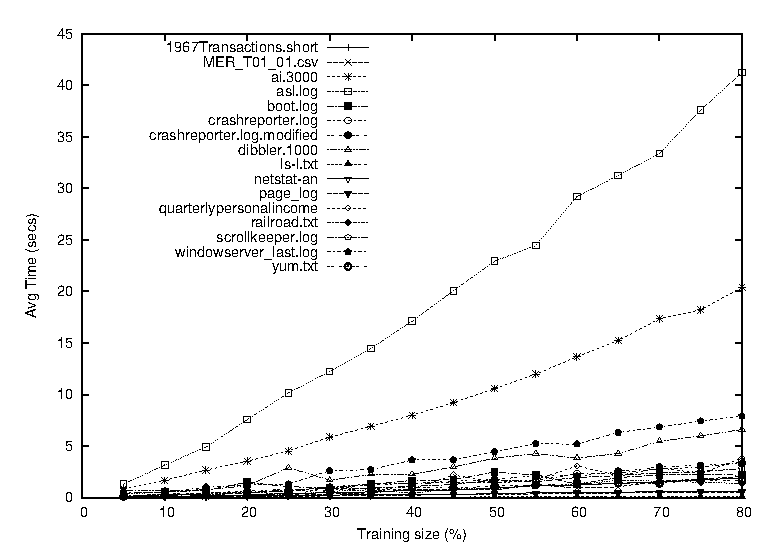
\epsfig{file=traintime.eps, width=\columnwidth}
\caption{Execution times of training sets}
\end{figure}

\begin{table}
\begin{center}
\begin{tabular}{|l|r|l|c|c|} \hline
Title 			& Bytes 	& Ty Comp	& 90\% 		& 95\% \\ \hline \hline
1967Transactions.short	& 70929		& 0.0003	& 5		& 5 			\\ \hline
MER\_T01\_01.csv        & 21731 	& 0.0037	& 5		& 5\\ \hline
ai.3000                 & 293460 	& 0.0004	& 5		& 10\\ \hline
asl.log                 & 279600	& 0.0012	& 5		& 10\\ \hline
boot.log                & 16241		& 0.0213	& 40		& 50\\ \hline
crashreporter.log       & 50152 	& 0.0052	& 5		& 5\\ \hline
crashreporter.log.mod   & 49255		& 0.0053	& 5		& 5\\ \hline
dibbler.1000            & 142607 	& 0.0001	& 5		& 5\\ \hline
ls-l.txt                & 1979		& 0.0461	& 50		& 70\\ \hline
netstat-an              & 14355		& 0.0118	& 20		& 25\\ \hline
page\_log               & 28170		& 0.0032	& 5		& 5\\ \hline
quarterlypersonalincome & 10177		& 0.017		& 10		& 20\\ \hline
railroad.txt            & 6218		& 0.0485	& 60		& 85\\ \hline
scrollkeeper.log        & 66288		& 0.002		& 5		& 5\\ \hline
windowserver\_last.log  & 52394		& 0.0084	& 5		& 10\\ \hline
yum.txt                 & 18221		& 0.0124	& 30		& 40\\ \hline
\end{tabular}
\caption{Min Training size (\%) vs. required accuracy}
\end{center}
\end{table}

\begin{figure}
\begin{center}
\epsfig{file=traintycomp.eps, width=\columnwidth}
\caption{Correlation between structure complexity of 
the data and minimum training size required}
\end{center}
\end{figure}
